\chapter{Theoretical Foundation}
\label{sec:related}
%

This chapter provides background information about ...
\todo{Describe Chapter}

\section{Scalability}
% What is scalability
Scalability defines the ability of a computing system to handle an increasing amount of load \cite{Farcic2017Toolkit21}.
% Why scaling
The main reasing for scaling is High-Availability TOOLKIT 2.1.
% Choose right approach
To choose the right approach of scaling an environment is essential.
% Different kind of scaling
To scale the computing capacity of a system, different approaches exists. A major scaling approach is horizontal scaling.

%% Mehr darüber, warum scaling eigentlich so wichtig ist, und welche probleme man damit löst


\subsection{Horizontal Scaling}
% What is horizontal scaling
Horizontal scaling is accomplished by duplicating nodes in the computing environment \cite{Wilder2012CloudPatterns}.
% DIstribution
Dplucation the nodes in a computing environment increases the computational capacity of the environment. In addition, the workload can be distributed across all clones to handle and balance and increasing load of tasks \cite{Wilder2012CloudPatterns, Abbott2015ScalabilityArt}. 
% What about homogeneous nodes
To increase the efficiency of horizontal scaling, all nodes should be homogeneous. Homogeneous nodes are able to perform the same work and response as other nodes \cite{Abbott2015ScalabilityArt}.


\subsection{Limitations of Scalability}
The limit of scalability is reached, when a computing system is not able to serve the requests of it`s concurrent users \cite{Wilder2012CloudPatterns}.
% hardware capacity
If the scalability of a computing environment is reached, an option is to add more powerful hardware resources to the system. This approach is called vertical scaling QULLE??. By adding more powerful hardware resources, the point can be reached, where more powerful hardware becomes unaffordable or not available \cite{Wilder2012CloudPatterns}.
% Why horizontal i recommended
To overcome the limits of hardware cpacity, a computing system shuld be designed to scale horizontally in the first place \cite{Abbott2015ScalabilityArt}.


% ===========================================
% ===========================================
\section{Autonomic computing}
\label{sec:02_autonomic_computing}
% What is autonomic computing
Autonomic computing is the ability of an IT infrastructure to automatically manage itself in accordance to high level objectives defined by administrators \cite{Kephart2003VisionComputing}.
% Why
Autonomic computing gives an IT infrastructure the flexibility to adapt dynamic requirements quickly and effectively to meet the challenges of modern business needs \cite{Murch2004Autonomic}. Therefore, autonomic computing environments can reduce operating costs, lower failure rates, make systems more secure and quickly respond to business needs \cite{Jacob2004AutonomicSolution}.


% What does it need
Computing systems need to obtain a detailed knowledge of it`s environment and how to extend it`s resources to be truly autonomic \cite{Murch2004Autonomic}.
% The 4 basic elements
An autonomic computing system is defined by four elements:
\begin{itemize}
\item \textbf{Self-configuring:}
Self-configuring refers to the ability of an IT environment to adapt dynamically to system changes and to be able to deploy new components automatically. Therefore, the system needs to understand and control the characteristics of a configurable item \cite{Murch2004Autonomic, Sinreich2006AnAB}.

\item \textbf{Self-optimizing:}
To ensure given goals and objectives, a self-optimizing environment has the ability to efficiently maximize resource allocation and utilization \cite{Jacob2004AutonomicSolution}. To accomplish this requirement, the environment has to monitor all resources to determine if an action is needed \cite{Murch2004Autonomic}.

\item \textbf{Self-healing:}
Self-healing environments are able to detect problematic operations and then perform policy-based actions to ensure that the systems health is stable \cite{Sinreich2006AnAB, Jacob2004AutonomicSolution}. The policies of the actions have to be defined and should be executed without disrupting the system \cite{Sinreich2006AnAB, Jacob2004AutonomicSolution}.

\item \textbf{Self-protecting:}
The environment must identify unauthorized access and threats to the system and automatically protect itself taking appropriate actions during its runtime \cite{Sinreich2006AnAB, Jacob2004AutonomicSolution}.
\end{itemize}


\subsection{Autonomic computing concept}

% Concept figure
\begin{figure}[h]%
\centering
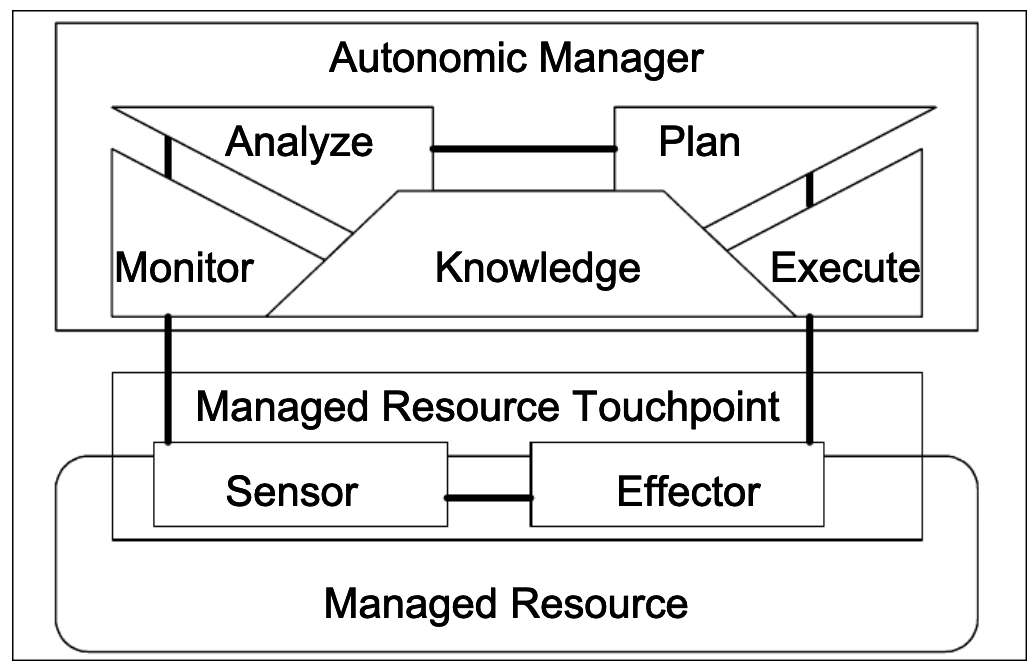
\includegraphics[scale=1]{images/04_technical_background/ac_concept}%
\caption{Autonomic computing concept - Source: Authors own model, based on \cite{Jacob2004AutonomicSolution}.}%
\label{fig:ac_concept}%
\end{figure}

% Figure + short description
\Fig{fig:ac_concept} demonstrates the main concept of an autonomic computing environment. The autonomic computing architecture relies on monitoring sensors and an adoption engine (autonomic manager) to manage resources in the environment \cite{Goscinski2011CloudComputing}.
% About the environment
In an autonomic computing environment, all components have to communicate to each other and can manage themselves. Appropriate decisions will be made by an autonomic manager that knows the given policies \cite{Jacob2004AutonomicSolution}.

% Control loop figure
\begin{figure}[h]%
\centering
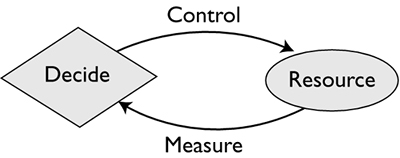
\includegraphics[scale=1]{images/04_technical_background/ac_control_loop}%
\caption{The control-loop concept - Source: Authors own model, based on \cite{Murch2004Autonomic}.}%
\label{fig:ac_control_loop}%
\end{figure}

% Explain control loop
The core element of the autonomic architecture is the control-loop. \Fig{fig:ac_control_loop} illustrates the concept of a control-loop. The control-loop collects details about resources through monitoring and makes decisions based on analysis of the collected details to adjust the system if needed \cite{Murch2004Autonomic}.


\subsection{Managed resources}

% Figure
\begin{figure}[h]%
\centering
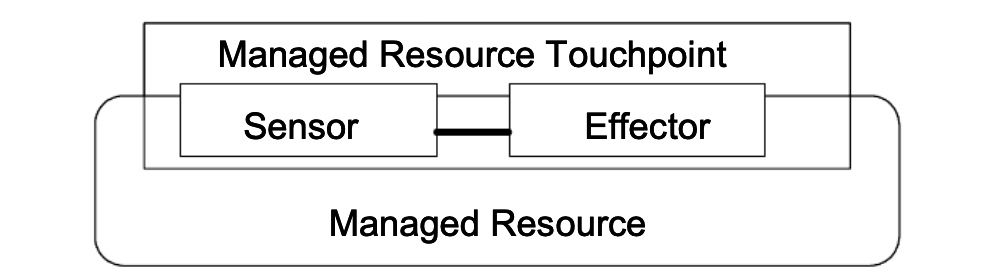
\includegraphics[scale=1]{images/04_technical_background/ac_managed_resource}%
\caption{Managed resource - Source: Authors own model, based on \cite{Jacob2004AutonomicSolution}.}%
\label{fig:ac_managed_resource}%
\end{figure}

% Explanation
A managed resource is a single component or a combination of components in the autonomic computing environment \cite{Murch2004Autonomic, Jacob2004AutonomicSolution}. A component can be a hardware or software component, e.g. a database, a server, an application or a different entity \cite{Sinreich2006AnAB}.
% Sensors and Effectors
They are controlled by their sensors and effectors, as illustrated in \Fig{fig:ac_managed_resource}. Sensors are used to collect information about the state of the resource and effectors can be used to change the state of the resource \cite{Jacob2004AutonomicSolution}. The combination of sensors and effectors is called a touchpoint, which provides an interface for communication with the autonomic manager \cite{Sinreich2006AnAB}.
% Scalability
The ability to manage and control managed resources make them highly scalable \cite{Murch2004Autonomic}.


\subsection{Autonomic manager}
\label{subsec:background-autonomic_computing-autonomic_manager}

% Figure
\begin{figure}[h]%
\centering
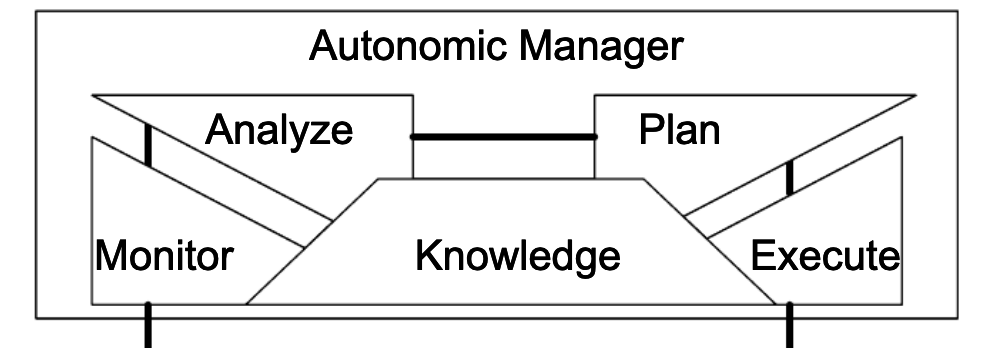
\includegraphics[scale=1]{images/04_technical_background/ac_autonomic_manager}%
\caption{Autonomic manager - Source: Authors own model, based on \cite{Jacob2004AutonomicSolution}.}%
\label{fig:ac_manager}%
\end{figure}

% WHat is the autonomic manager
The autonomic manager implements the control-loop to collect, aggregate, filter and report system metrics from the managed resources. It can only make adjustments within it`s own scope and uses predefined policies to make decisions of what actions have to be executed to accommodate the goals and objectives \cite{Murch2004Autonomic, Sinreich2006AnAB}.
% Knowledge
In addition, the autonomic manager gains knowledge through analyzing the managed resources \cite{Murch2004Autonomic}.
% MAPE-K
The autonomic computing concept digests the MAPE-K model to implement an autonomic manager, as illustrated in \Fig{fig:ac_manager} \cite{Goscinski2011CloudComputing}.

\begin{itemize}
\item \textbf{Monitor:}
The monitor phase is responsible to collect the needed metrics from all managed resources and applies aggregation and filter operations to the collected data \cite{Sinreich2006AnAB}.

\item \textbf{Analyze:}
The autonomic manager has to gain knowledge to determine if changes have to made to the environment \cite{Sinreich2006AnAB}. To predict future situations, the autonomic manager can model complex situation given the collected knowledge \cite{Jacob2004AutonomicSolution}.

\item \textbf{Plan:}
Plans have to be structured to achieve defined goals and objectives. A plan consists of policy-based actions \cite{Jacob2004AutonomicSolution, Sinreich2006AnAB}.

\item \textbf{Execute:}
The execute phase applies all necessary changes to the computing system \cite{Sinreich2006AnAB}.
\end{itemize}

% Multiple manager
Multiple autonomic manager can exist in an autonomic computing environment to perform only certain parts. For example, there can be one autonomic manager which is responsible to monitor and analyse the system and another autonomic manager to plan and execute. To create a complete and closed control-loop, multiple autonomic manager can be composed together \cite{Sinreich2006AnAB}.


% ===========================================
% ===========================================
\section{System Performance}


\subsection{Performance Metrics}
% Short description
Performance metrics are statistics that describe the system performance. These statistics are generated by the system, applications or other tools \cite{Greg2020SysPerf}.
% Common types
The following are examples of common types for performance metrics:
\begin{itemize}
\item \textbf{Throughput:} Volume of data or operations per second \cite{Greg2020SysPerf}.
\item \textbf{Latency:} Time of operation \cite{Greg2020SysPerf}.
\item \textbf{Utilization:} Usage of a component \cite{Greg2020SysPerf}.
\end{itemize}


% Overhead
\paragraph{}Measuring performance metrics can cause an overhead. To gather and store performance metrics, CPU cycles must be spent. This can have a negative affect on the target performance \cite{Greg2020SysPerf}.


\subsection{Time-Based Utilization}
% What is utilization
Utilization is a performance metrics that describes the usage of a device, e.g. CPU device usage.
% What about time-based utilization
A time-based utilization describes the usage of a component during a time period where the component was actively performing work \cite{Greg2020SysPerf}.
% 100% utilization
When a resource approaches 100\% utilization, the performance of that resource can degrade. If a component can process operations in parallel, the performance does not have to degrade much at 100\% utilization and the component can process more work \cite{Greg2020SysPerf}.


% ===========================================
% ===========================================
\section{Monitoring}
% What is monitoring
Monitoring is a process, that aims to detect and take care of system faults. In a dynamic environment, becoming aware of the system is trivial \cite{Ligus2012EffMonitoring}.
% What is a monitoring system
A monitoring system consists of a set of different tools. The tools are responsible to perform measurements on components in the computing environment and collect, store and interpret the monitored data \cite{Ligus2012EffMonitoring}. 


% The monitoring Loop/Process
\begin{figure}[h]
\centering
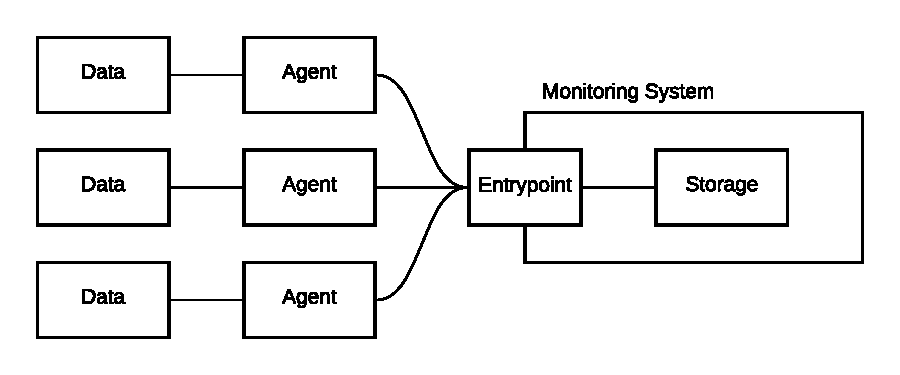
\includegraphics[scale=0.9]{images/02_theoretical_foundation/monitoring/monitoring_system}
\caption{The monitoring process - Source: Authors own model.}
\label{fig:mon_mon-system-process}
\end{figure}
In the monitoring process, illustrated in \Fig{fig:mon_mon-system-process}, data is continuously collected by agents. An agent is a process that continuously gathers metrics. Data can be device statistics, logs or system measurements. Agents will group these data into metrics and submit them to the monitoring system via a protocol. The monitoring system will store the metrics in its database \cite{Ligus2012EffMonitoring}.


% Requirements of a monitoring system
The requirements for a monitoring system, that is able to monitor a dynamic changing environment, are the following:
\begin{itemize}
\item An efficient database to store metrics
\item A decentralized way of generating metrics \cite{Farcic2017Toolkit21} % Neu schreiben
\item Multi-dimensional metrics \cite{Farcic2017Toolkit21}
\item A powerful query language \cite{Farcic2017Toolkit21}
\end{itemize}


\subsection{Database}
% TS are needed
Saving continous data needs to be done efficiently. 
For time-based metrics, a time series database is he most effective way to save the data \cite{Farcic2017Toolkit21}. To store a huge amount of data, data is stored in a very compact format.
A BISL MEHR ÜBER METRICS UND TIMESERIES.


\subsection{Decentralized Way of gathering Metrics}
The approach how the monitoring systems gathers metrics to store in the database plays a significant role.
% There are push and pull based systems
Push and pull based systems are the two primary approaches to gather metrics from services.
% About push
Push based monitoring systems expect services to push metrics to their storage.
% About pull
On the other hand, pull based monitoring systems scrape metrics from all defined targets. Targets do not know about the existence of the monitoring system and only need to collect and expose metrics.


% When to choose what (Discovery)
Service discovery is an important aspect to decide whenever to use a pull or push based monitoring system.

\begin{figure}[h]
\centering
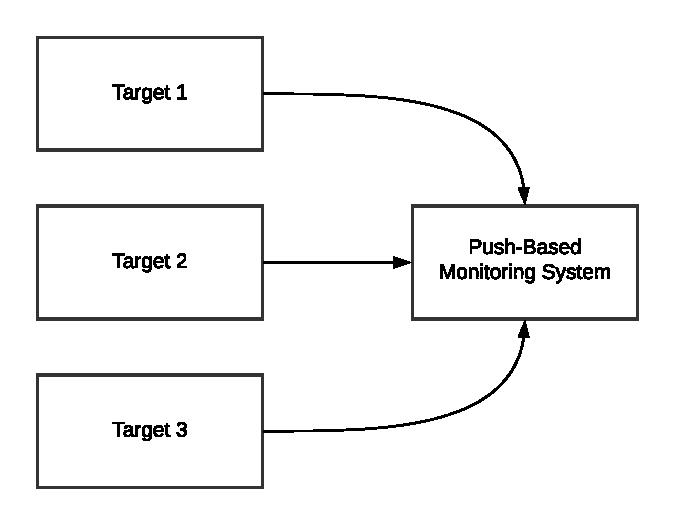
\includegraphics[scale=0.8]{images/02_theoretical_foundation/monitoring/push_based}
\caption{Push-based monitoring approach - Source: Authors own model.}
\label{fig:mon_push-based}
\end{figure}
% Push based discovery
In a push-based environment, services only need to know the address of the monitoring service to push their data to the storage.


\begin{figure}[h]%
\centering
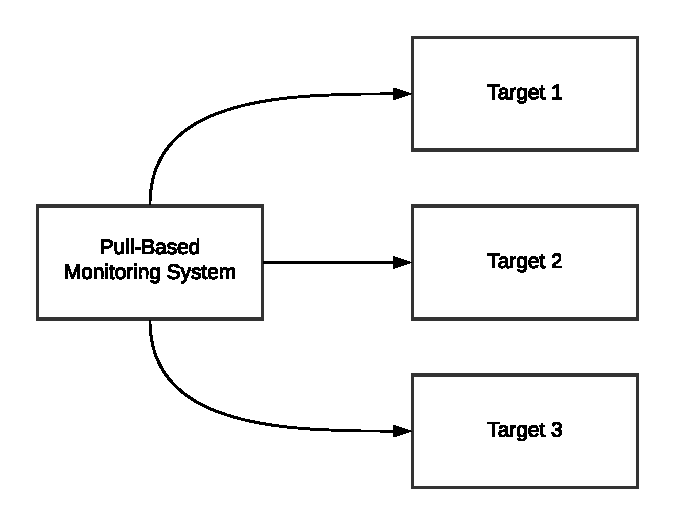
\includegraphics[scale=0.8]{images/02_theoretical_foundation/monitoring/pull_based}%
\caption{Pull-based monitoring approach - Source: Authors own model.}%
\label{fig:mon_pull-based}%
\end{figure}
% Pull based discovery
A pull-based monitoring tool needs to know the address of each target in the environment.
% Why pull based works best with discovery
The advantage of a pull-based systems are, they know what they expect. It is ieasier for pull-based monitoring system to detect whenever a target has failed or is not available.


\subsection{Multi-dimensional Metrics}
% Why do we need dimensions
For query languages to be effective, metrics need to be dimensional. Metric without dimensions, are limited in their capabilities.
% Dynamic environment
In a dynamic environment, services are dynamically added and removed. Therefore, a dynamic environment needs dynamic analytics where metrics represent all dimension in the environment \cite{Farcic2018Toolkit22}.
% Example
\begin{lstlisting}[frame=single, label=lst:mon_metr_dimless, caption=Example of a dimensionless-metric, captionpos=b]
container_memory_usage
\end{lstlisting}
\begin{lstlisting}[frame=single, label=lst:mon_metr_withdim, caption=Example of a metric with dimensions, captionpos=b]
container_memory_usage{service="my_service"}
\end{lstlisting}
% Explain
As the exasmple \Lst{lst:mon_metr_dimless} and \Lst{lst:mon_metr_withdim} show, the metric with dimension provide more efficient querieing to gather informations about the environment.


\subsection{Query Language}



\subsection{Choosing a Monitoring Tool}
Graphite or Prometheus, Prometheus it its! <- Eher in Design
